\section{Cooperation}\label{Scrum/agile-cooperation}
\textit{The following sections is written in collaboration with other ECDAR project groups.}




\begin{comment}
%Introduction to the concept of this semester project and the fact that we are continuing development of an existing program:
This semester project specifically focuses on multi-project cooperation, which means that several project groups will be cooperating on the same project. In total, six project groups consisting of six members each will be cooperating to further extend ECDAR. Five of these groups will be focusing on further development of the Reveaal engine, while the last group will focus on development of the graphical user interface of ECDAR. However, all six groups....


\end{comment}




The ECDAR project is a newly started project and therefore there have not been any iteration of the project.
For the first iteration the groups first job was to startup everything collaborative related. 
The way the groups could uphold knowledge sharing was by planning scrum meetings.

There were six project groups that chose ECDAR as their semester project. 
Five groups that choose to work with the reveaal engine and one group that choose the graphical user interface engine.
%Because there were so many students working on the ECDAR project the scrum meetings would get too big if every group member attended the meetings.
%Based on that the groups choose a committee to attend the scrum meetings.


%Har tilføjet det her -Christian


\subsection{The ECDAR-SW5 Organization}
There must be some kind of organization in order to orchestrate collaboration between all the project groups that are working on the ECDAR project. 
Organization is important because it establishes channels of communication, a distribution of the workload, and a process for evaluating the outcome of each stage in the development process.

All of the project groups that are a part of the ECDAR-SW5 organization are themselves a scrum team. 
As scrum is dependent on the teams being small, the organization must use an agile scaling framework. 
Such a framework ensures distribution of the workload between the teams and that the output from each team can be integrated. 
As agile is very popular within some of the largest organizations in the world(SOURCE PLEASE), multiple different agile scaling frameworks have been invented. 
When an organization needs to pick a framework to implement, it must consider its needs. 
The groups that make up the ECDAR-SW5 organization must be self-managed and free to decide how they work internally. They have responsibility for their own project after all. The organization has to choose a framework that allows teams this flexibility.


\subsection{Scrum of scrums}
Scrum of Scrums is a framework for scaling scrum across an organization. It allows each scrum team freedom to operate while providing a structure for communicating progress. 

In the ECDAR project the term scrum of scrums was introduced to cooperate transparency between the groups.
In scrum of scrums we do not have daily scrums because the daily scrums is hold in the smaller groups.
The key events in scrum of scrums are the sprint planning sprint review and sprint retrospective.
Look at \autoref{fig:scrum-of-scrums-events} for a more detailed look of the different events between scrum and scrum of scrums.


Because there were so many students working on the ECDAR project the scrum meetings would get too big if every group member attended the meetings.
Based on that the groups choose a committee to attend the scrum meetings.

\begin{figure}[H]
    \centering
    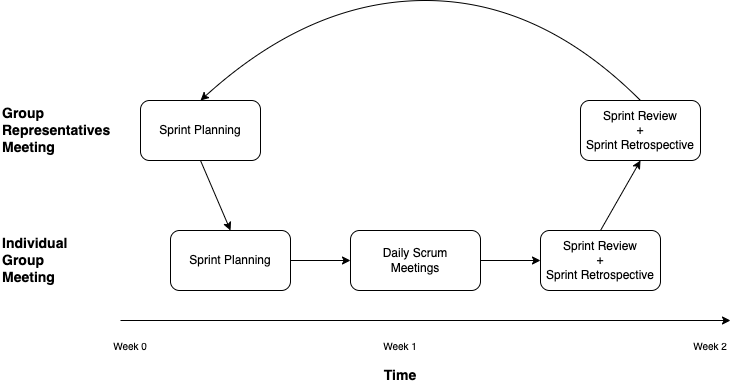
\includegraphics[width=\textwidth]{common/figures/Scrum_of_scrums_schedule.png}
    \caption{The events in a scrum sprint divided between the big scrum of scrums group and the smaller scrum groups}
    \label{fig:scrum-of-scrums-events}
\end{figure}


The multi project is separated in two parts. 
There are five project groups working on the Reveaal part and one group working on the GUI part.
Because of this we have two product owners.
One product owner for the Reveaal part and one for the GUI part.




\subsection{Shared tools for collaboration}
For every group in the scrum groups there are a shared toolbox.
This toolbox contains tools that helps the groups cooperate between groups.
The main tool is Github and it is used for version management.  
Each group have their own repository and if the groups shares the same repository then they have individual branches.
Because of this a branching strategy was made on the first meeting in the scrum of scrums.
For each increment a branch is made from the main branch on the specific repository. 
When a increment is done, tested and reviewed the branch can be merged back into the main branch.

To keep track of increments and the backlog a project board is used on Github.
This board holds all the information of the different increments the individual groups works on.

To communicate between groups a discord server was created.
The server contains different text channels that are used for different purposes e.g a channel for the joint writing sections and a channel for setting up meetings.

For every meeting in the scrum of scrums a agenda is created and distributed between the groups through a OneDrive.
The OneDrive is also used for sharing documents, notes etc..

The joint writing is done in Overleaf and later uploaded to Github in a repository.
This makes i possible to write together in real time and later inserted into the individual group's report.
This concludes the section of the shared tools.